

\begin{figure}[!ht]
    \centering
    
    % 第一张图
    \subfloat[Performance on XES3G5M]{
        % 使用 width=0.48\linewidth 代替 scale，确保两张图加起来不超过 1，刚好并排
        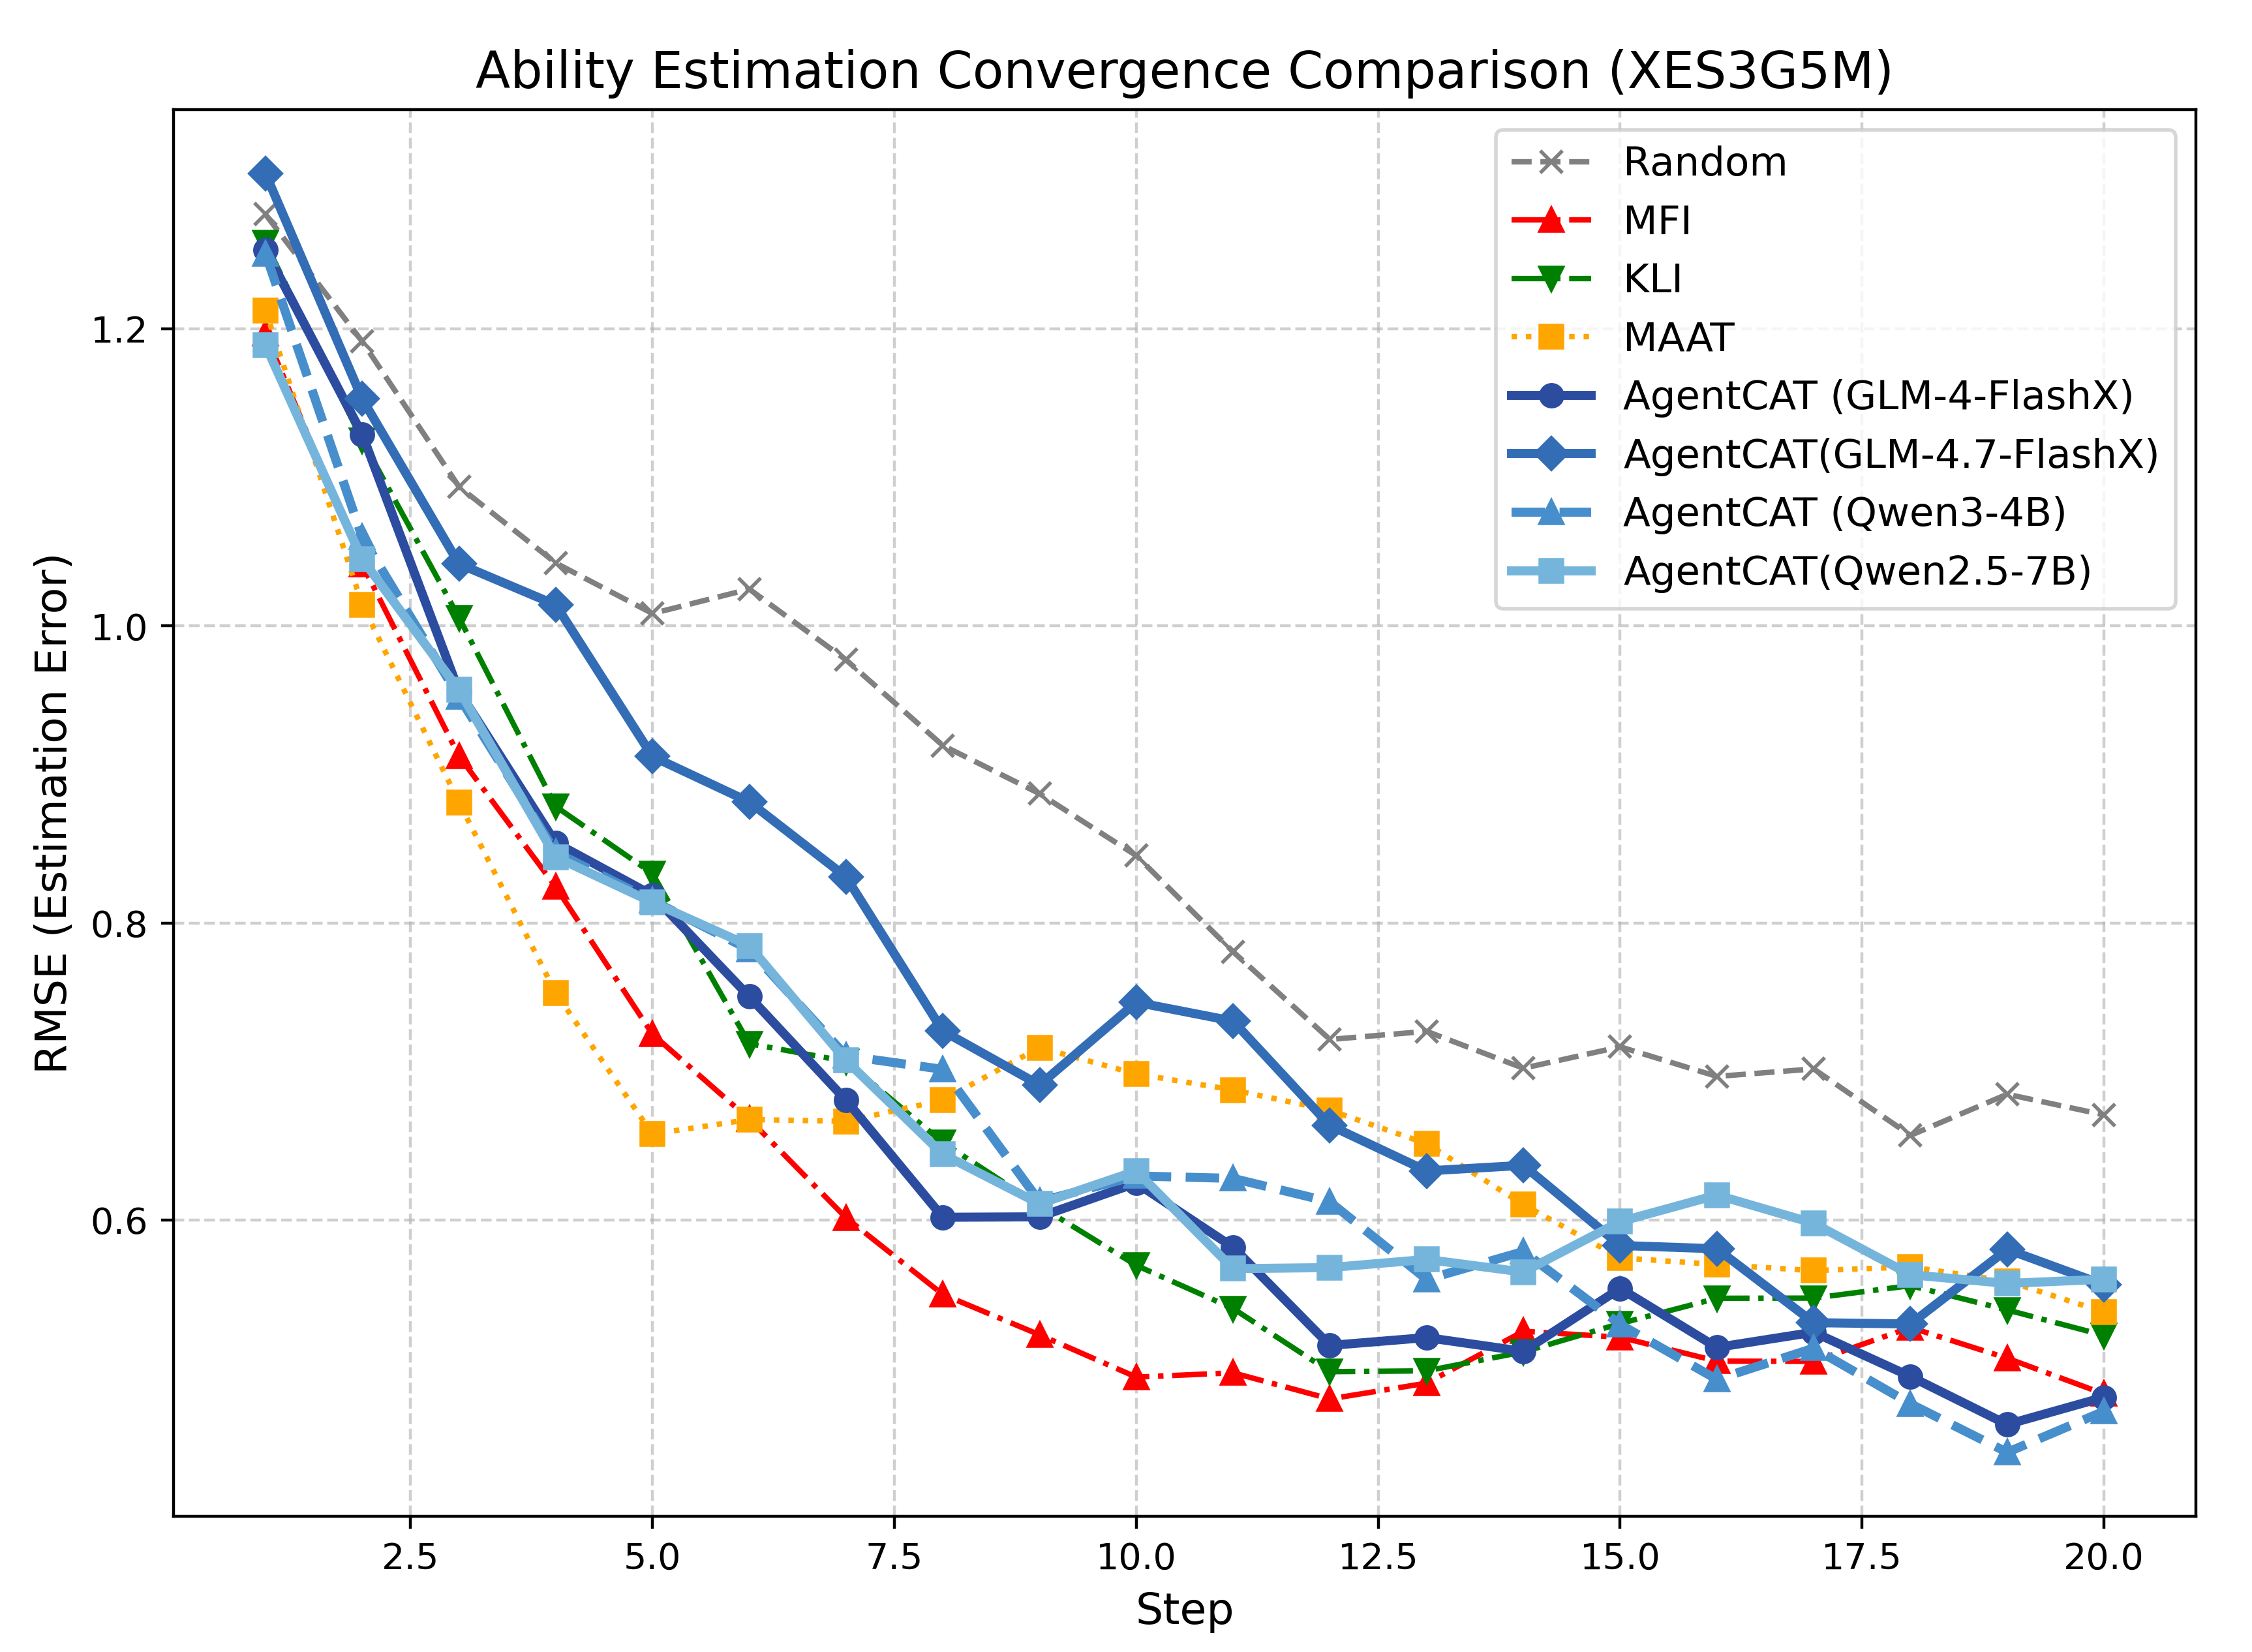
\includegraphics[width=0.48\linewidth]{acmart-primary/samples/Figure/image/exp1_XES3G5M_V2.png}
        \label{fig:rmse_xes}
    }% 这里不要留空行！
    \hfill % \hfill 会在两张图中间自动填充水平空白，把它们向两边推开
    % 第二张图
    \subfloat[Performance on C\_797404]{
        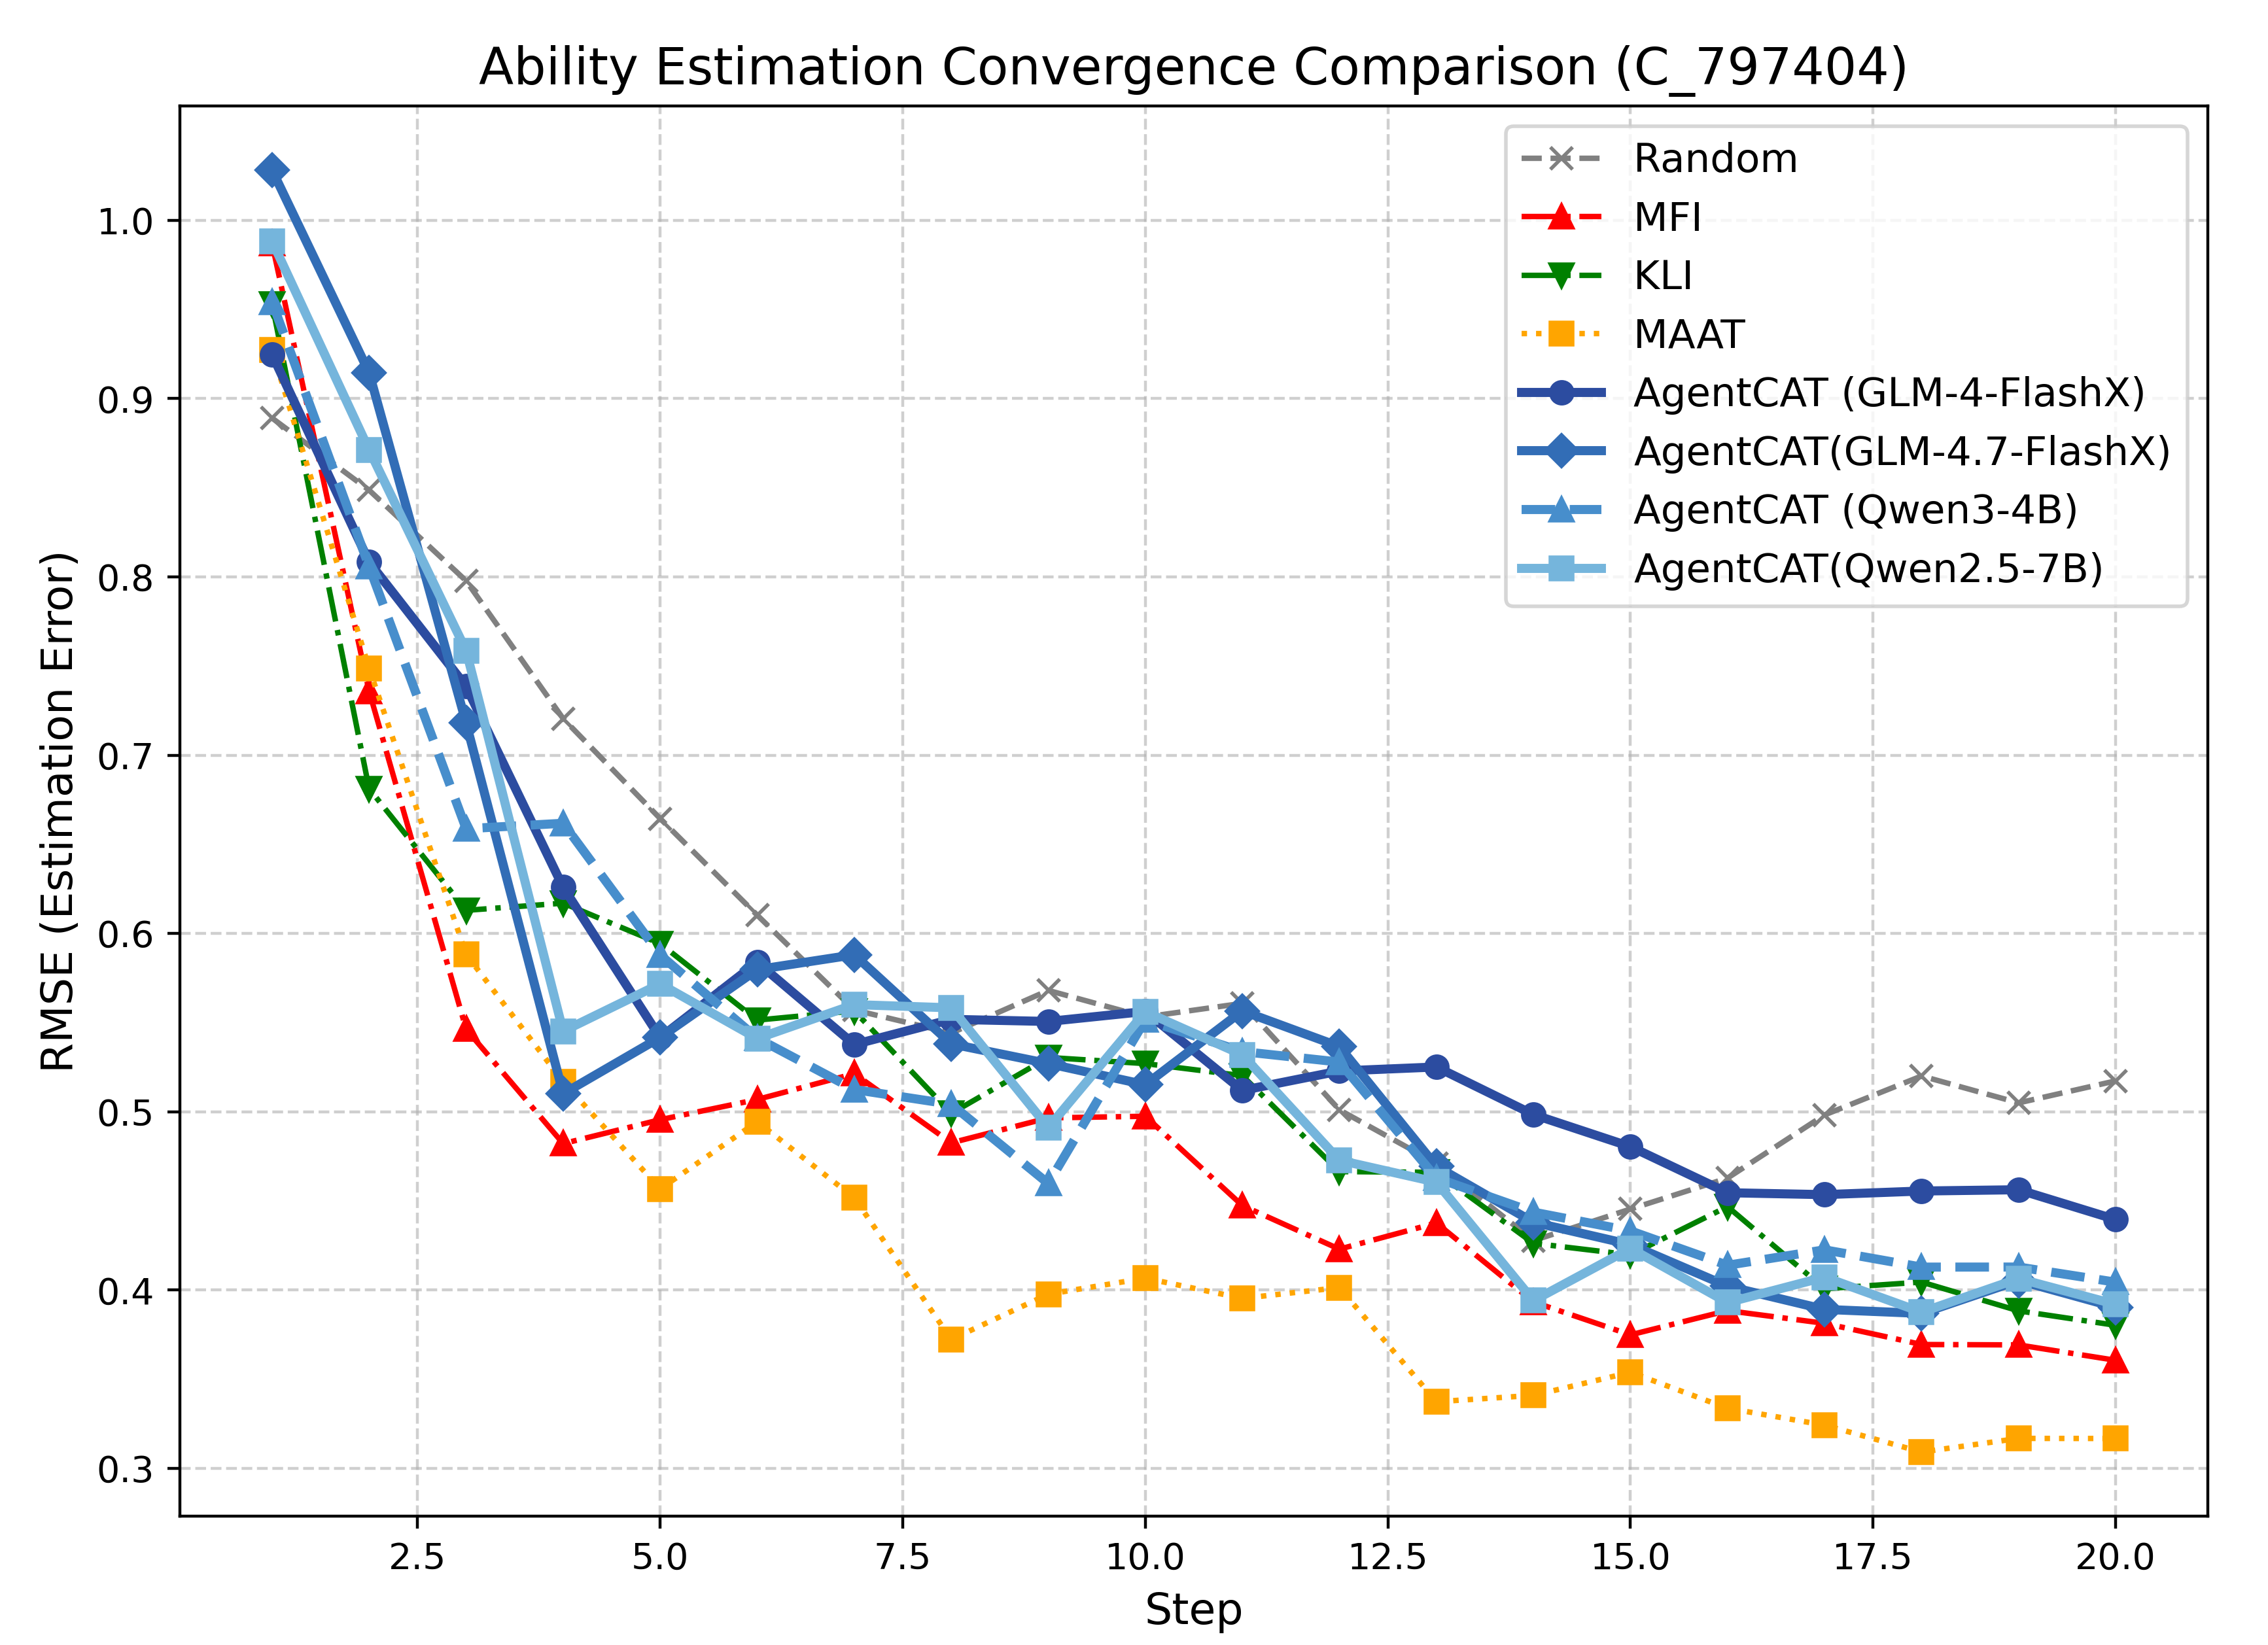
\includegraphics[width=0.48\linewidth]{acmart-primary/samples/Figure/image/exp1_797404_V2.png}
        \label{fig:rmse_mooc}
    }
    
    % 总标题
    \caption{Ability estimation convergence comparison (RMSE) on two datasets. AgentCAT demonstrates consistent convergence trends comparable to classical mathematical baselines across different LLMs backbones.}
    \label{fig:rmse_convergence}
\end{figure}
